\begin{frame}{古中国数学}{定理证明}
有论者认为早在公元前 11 世纪商高即已证明勾股定理\cite{quanjing}。
完整的证明见于三国时(公元 3 世纪)赵爽对《周髀算经》的注释。
\begin{figure}
\centering
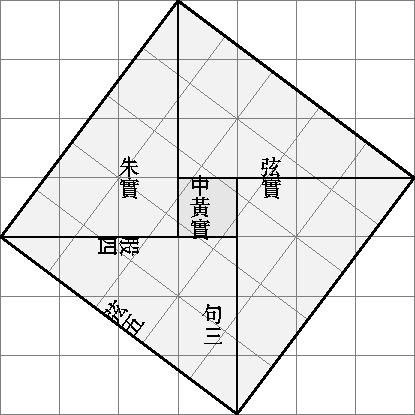
\includegraphics[height=0.4\textheight]{xiantu.pdf}
\caption{赵爽的弦图可给出勾股定理的一个富于对称美的证明}
\end{figure}
\end{frame}
